\section{Protocolli dello strato di trasporto}
    Abbiamo indagato lo strato fisico, di collegamento e di rete: passiamo quindi allo strato di trasporto.
    
    \vspace{3mm}
    
    Lo \textbf{strato di trasporto} si occupa della consegna di un messaggio da un processo mittente ad un processo destinatario. 
    
    \vspace{3mm}
    
    Nei capitoli precedenti, abbiamo visto che l'IP permette, sì, lo scambio di messaggi fra due nodi, ma in maniera inaffidabile, cioè non garantendo che i messaggi stessi arrivino a destinazione. 
    
    E' dunque necessario aggiungere allo strato di rete la proprietà di affidabilità e la possibilità di scambiare informazioni fra processi diversi (e non semplicemente nodi) - questi sono i motivi che hanno portato alla creazione dello strato di trasporto.
   
    \vspace{3mm}
   
    Lo strato di trasporto offre differenti protocolli al fine di permettere ai processi di comunicare fra di loro.
   
    \begin{itemize}
        \item 
            \textbf{User Datagram Protocol (UDP).} Senza garanzia di consegna dei pacchetti.
            
        \item
           \textbf{Transmission Control Protocol (TCP).} Con garanzia di consegna dei pacchetti.
            
        \item
            \textbf{Stream Control Transmission Protocol (SCTP).} Utilizzato per i flussi di dati audiovisivi. Combina caratteristiche di UDP e TCP, offrendo anche nuove funzionalità.
    \end{itemize}
   
    A livello di collegamento, si ha una comunicazione nodo-nodo.
   
    A livello di rete, si ha una comunicazione host-host (che significa "nodo-nodo" ma non per forza direttamente collegati).
   
    A livello di trasporto, si ha una comunicazione processo-processo.
   
    \subsection{Caratteristiche dello strato di trasporto}
   
    In generale, lo strato di trasporto offre una serie di servizi, come l'indirizzamento dei numeri di porta, l'incapsulamento/decapsulamento, il multiplexing/demultiplexing, il controllo del flusso, della congestione e degli errori, e ovviamente la comunicazione fra processi. 
    
    Inoltre, offre sia servizi orientati alla connessione, che servizi privi di connessione.
   
        \subsubsection{Comunicazione fra processi}
       
            Oltre all'indirizzo IP, abbiamo bisogno di un ulteriore meccanismo che ci permetta di individuare il processo sull'host: il \textbf{numero di porta}. Si tratta di un intero fra 0 e 65535. Due numeri di porta permettono una comunicazione bidirezionale.
           
            \vspace{3mm}
           
            Quasi tutte le applicazioni di rete che vengono progettate seguono il modello client/server. Di solito vi è un server perennemente in esecuzione e un numero di client variegati che richiedono un servizio al server. E' il client che richiede il servizio (e quindi inizia la comunicazione), mentre il server si limita a restituire il risultato.
           
            Osserviamo che i numeri di porta sono necessari tanto sul processo mittente quanto su quello destinatario. Quindi abbiamo bisogno di quattro informazioni:
           
            \begin{itemize}
                \item 
                    \textbf{Host locale} (indirizzo IP del client)
                    
                \item
                    \textbf{Host remoto} (indirizzo IP del server)
                    
                \item
                    \textbf{Processo locale} (numero di porta del client)
                    
                \item
                    \textbf{Processo remoto} (numero di porta del server)
            \end{itemize}
        
        \subsubsection{Indirizzi di porta}
        
            Lo strato di trasporto deve instradare il client verso il corretto processo remoto. 
            
            \vspace{3mm}
            
            Facciamo un esempio pratico: dai livelli più bassi (fisico, collegamento) arriva un certo pacchetto. 
            
            Al livello di rete, l'indirizzo IP del destinatario identifica l'host remoto (cioè il server) e passa il pacchetto allo strato di trasporto, che riceve il messaggio (il quale prende il nome di \textit{datagram} se si parla di UDP, o \textit{segmento} se si parla di TCP) e ne estrae l'header per capire a quale processo deve mandare i dati - il numero di porta ottenuto identifica il processo applicativo, che viene impiegato infine nello strato di applicazione, concludendo (finalmente!) la comunicazione.
            
            \vspace{3mm}
            
            I server girano su porte ben note. Ad esempio la 80 (\underline{web}), 25 (email), 22 (SSH), 13 (daytime).
            
            I client girano, invece, su \textit{porte effimere}, poiché hanno una vita breve, limitata funzionalmente alla comunicazione in atto. Sono scelte a caso.
            
            \vspace{3mm}
            
            Esiste un'agenzia, la IANA (Internet Assigned Number Authority), preposta all'assegnazione dei numeri di porta. Le porte fra 0 e 1023 sono riservate, quelle da 1024 a 49152 si possono "registrare" e le successive fino a 65535 si possono usare liberamente. 
            
            In parole povere, se voglio installare un nuovo servizio personalizzato sul mio server, e su questo server ci gira Tomcat, e imposto la porta del servizio (che ricordiamo corrisponde ad una \textit{applicazione}) a 80, allora si verificherà un conflitto, dato che Tomcat è un webserver.
        
        \subsubsection{Socket Address}
        
            Il \textbf{Socket Address} (o semplicemente \textit{Socket}) identifica univocamente un processo con la combinazione indirizzo IP e indirizzo di porta. 
                
            \vspace{3mm}    
            
            Per una comunicazione client-server avremo bisogno di un socket per il client e di un socket per il server. Le informazioni relative a entrambi i socket sono parte dell'instazione di un datagram P e dell'intestazione aggiunta dal protocollo di trasporto. Ricordiamo che il datagram IP contiene gli indirizzi IP della sorgente e della destinazione, mentre l'intestazione del protocollo di trasporto contiene i numeri di porta.
        
        \subsubsection{Multiplexing Client-Server}
        
            Nell'host mittente possono esserci vari processi che spediscono dati. Tutti i processi vogliono utilizzare il servizio di comunicazione offerto dallo strato di rete, che è unico. Lo strato di trasporto deve effettuare il multiplexing dei dati in arrivo dai vari processi, assegnando un numero di porta ad ogni processo e aggiungendo tale numero in una intestazione per idati in arrivo dal processo, spedendo infine i dati utilizzando lo strato di rete.
            
            \vspace{3mm}
            
            Sull'host di destinazione vengono consegnati tutti i datagram destinati a qualsiasi processo attivo sull'host di destinazione. Lo strato di trasporto della destinazione, grazie al numero di porta inserito nell'instazione creata dallo strato di trasporto nel mittente, consegna correttamente i datagram ai processi di destinazione.
    
        \subsubsection{Controllo del flusso}
        
            \textit{Controllare il flusso} significa fare attenzione a produrre una quantità di dati tale che il destinatario riesca a gestirne la mole. Basti notare che la velocità di produzione (invio dei dati) lato client potrebbe essere più veloce rispetto alla controparte server.
            
            \vspace{3mm}
            
            Se la velocità di produzione è maggiore della velocità di consumo, il destinatario potrebbe essere sovraccaricato e costretto ad eliminare alcuni dati.
            
            Se la velocità di produzione è minore della velocità di consumo, il destinatario rimane in attesa riducendo l'efficienza del sistema.
            
            \vspace{3mm}
        
            L'obiettivo è evitare di perdere dati. Questo è il famoso "\textit{traffico}".
            
            La gestione del controllo del flusso è duplice, cioè lato applicativo server e lato applicativo client. In termini pratici, se lo strato di applicazione del mittente produce dati troppo velocemente, lo strato di trasporto del mittente gli chiederà di rallentare. Tale controllo è speculare nel destinatario.
            
            \begin{center}
                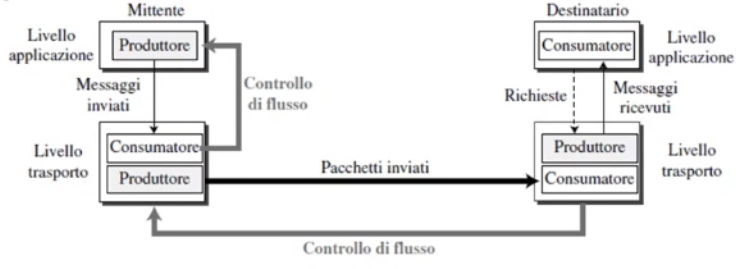
\includegraphics[scale=0.5]{images/ControlloFlusso.png}
            \end{center}
            
            Una soluzione per realizzare il controllo di flusso sono i cosiddetti \textbf{buffer}, definiti come un insieme di locazioni di memoria che possono contenere pacchetti. Se il buffer è saturo, l'invio o la ricezione dei dati si interrompe.
            
        \subsubsection{Controllo degli errori}
        
            Bisogna scartare i pacchetti corrotti, riconoscere pacchetti duplicati (usando i \textit{numeri di sequenza}), tenere traccia dei pacchetti persi (usando i \textit{numeri di riscontro}, cioè gli ACK) ed eventualmente richiederne il rinvio. Per avere un servizio di trasporto affidabile è necessario implementare un controllo degli errori. Il protocollo UDP ha difficoltà (o quasi totale incapacità) a controllare gli errori, a differenza del TCP.
            
            \vspace{3mm}
            
            Controllo del flusso e controllo degli errori viaggiano sempre in coppia. Il controllo del flusso richiede due buffer, mentre il controllo degli errori richiede il numero di sequenza e il numero di riscontro. La combinazione dei due meccanismi è detto \textbf{buffer numerato} (uno per il mittente, uno per il destinatario).
            
            \vspace{3mm}
            
            Sul mittente, quando un nuovo pacchetto viene preparato allora gli verrà assegnato il numero di sequenza $x$ e occuperà l'$x$-esima posizione nel buffer - in questo modo c'è una sorta di specchio fra "posizione nel buffer" e "identificativo del pacchetto". Quando il mittente invia un pacchetto, ne memorizza una copia nel buffer alla locazione $x$; infine, quando il mittente riceverà un'ACK da un pachetto, libera la posizione di memoria occupata da quel pacchetto.
            
            In maniera analoga, il destinatario memorizzerà nel buffer alla locazione $y$ il pacchetto con numero di sequenza $y$ fin quando il livello di applicazione non è pronto a riceverlo. Quando il pacchetto $y$ passa al livello di applicazione, il destinatario invia un ACK al mittente.
            
            \vspace{3mm}
            
            Poiché i numeri di sequenza sono calcolati in modulo $2^m$, questi buffer sono rappresentabili come un insieme di settori, chiamati \textbf{finestre scorrevoli}, che in ogni istante occupano una parte di un immaginario cerchio.
            
        \subsubsection{Servizo di comunicazione}
        
            In generale, un protocollo può offrire un servizio di comunicazione orientato o meno alla connessione - non è un'esclusiva dello strato di trasporto. In ogni caso, i protocolli di trasporto offrono entrambi i servizi.
            
            \vspace{3mm}
            
            Un servizio non orientato alla connessione, utilizzato dall'UDP, prevede che i dati siano spediti immediatamente, senza che client e server abbiano già instaurato una connessione fra di loro. I datagram così non saranno numerati, saranno spediti in maniera indipendente e non vi sarà relazione fra di loro, arrivando quindi in modo disordinati
            
            Un servizio orientato alla connessione, utilizzato da TCP e SCTP, prevede una previa instaurazione della connessione fra client e server. I datagram "\textit{appartengono}" alla connessione, motivo per cui vi è una relazione fra i dati. L'idea è che, prima di inviare i dati, client e server debbano mettersi d'accordo sull'invio dei \textit{messaggi di sincronizzazione}, sui quali ritorneremo. Alla fine della comunicazione, la connessione viene chiusa.
            
            \vspace{3mm}
            
            E' palese che l'UDP sia quindi più veloce (proprio perché non deve stabilire una connessione prima di spedire i dati). Il TCP, invece, deve spedire 4 segmenti per instaurare la connessione e altrettanti per chiuderla. Tuttavia, TCP è affidabile, mentre UDP non lo è.
            
            \vspace{3mm}
            
            Un'applicazione interessata ad utilizzare un servizio non orientato alla connessione è, ad esempio, lo streaming di servizi multimediali, dato che in questo caso si tratta di un "rischio ragionato e ragionevole" - la perdita di pacchetti corrisponderebbe alla perdita dei frame dei video, che nel contesto di una riproduzione di quel tipo "non è una grande perdita". 
            Un servizio orientato alla connessione è invece imperativo in applicazioni che riguardano le transazioni bancarie.
            
            \vspace{3mm}
            
            Lo strato di collegamento e di rete già prevedono sistemi di controllo di flusso e degli errori. Perché dobbiamo anche offrirli a livello di trasporto? Banalmente, ricordiamo che lo strato di collegamento offre affidabilità nell'ambito della comunicazione fra due nodi, ma il protocollo IP allo strato di rete non è affidabile, pertanto è possibile che i pacchetti vengano persi, eliminati o danneggiati durante il passaggio in un router.
            
        \subsubsection{Accenni al controllo della congestione}
        
            Non sono solo gli host a poter essere congestionati, cioè sovraccaricati, ma anche la rete stessa. Questo avviene perché i router non riesce ad elaborare i pacchetti alla stessa veloca con la quale sono stati spediti. Un router sovraccarico sarà costretto a resettare le connessioni.
            
            Indagheremo il controllo della congestione nei prossimi capitoli.
            
    \subsection{User Datagram Protocol}
    
        Senza connessione e inaffidabile, quindi molto simile ad IP. Offre la comunicazione fra processi tramite i numeri di porta; tuttavia, non fornisce alcun controllo del flusso, degli errori (eccetto la somma di controllo) e della congestione. Ha il vantaggio di essere molto efficiente.
        
        Definiamo il formato di una datagram UDP, la cui intestazione è lunga 8 byte, ed è composta come segue.
        
        \begin{itemize}
            \item
                \textbf{Lunghezza (16 bit).} Definisce la lunghezza totale del datagram, inclusi header e dati. Si potrebbe lecitamente pensare che questo campo non sia necessario, poiché il datagram IP (in cui è incapsulato il datagram UDP) conterrà - nella propria intestazione - la lunghezza di ambo i datagram. Tuttavia, ciò non è del tutto esatto.
                
                Nel mittente, ancora non abbiamo i dati forniti dall'intestazione del datagram IP (lo strato di trasporto viene prima dello strato di rete!), mentre nel destinatario abbiamo già "estratto" le informazioni dell'header IP, motivo per cui questo campo è in realtà necessario.
                
            \item
                \textbf{Numero di porta del mittente (16 bit).}
                
            \item
               \textbf{Numero di porta del destinatario (16 bit).}
                
            \item
                \textbf{Somma di controllo (16 bit).} Dedicata al controllo degli errori. Il calcolo avviene su una pseudointestazione (contenente indirizzo IP mittente, indirizzo IP destinatario, e altri valori), l'intestazione del datagram UDP e sui dati.
        \end{itemize}
        
        \subsubsection{Code di entrata e uscita}
        
            Quando un processo client richiede l'utilizzo di un determinato servizio, viene assegnato un numero di porta al processo e vengono create delle opportune code in entrata e uscita (i buffer) in cui mantenere i messaggi.
            
            In parole povere, i buffer vengono allocati in maniera concorrente agli indirizzi di porta.
            
            Appena il processo termina, le code vengono elimiante, e la porta viene restituita al pool di porte libere. Osserviamo che sia client che server hanno due code (una in entrata e una in uscita), quindi le code sono complessivamente 4.
            
            \vspace{3mm}
            
            Se una delle code non esiste, l'UDP elimina il datagram e chiede al protocollo ICMP di spedire un messaggio di porta non raggiungibile. Una coda potrebbe risultare inesistente, ad esempio, perché si sta tentando di indirizzare una porta sbagliata.
             
            E' importante sottolineare che i messaggi arrivano all'interno delle code a prescindere dal processo destinatario, e tramite il demultiplexing viene determinato in quale processo deve proseguire un certo messaggio.